\documentclass[12pt]{My_preprint}

\usetikzlibrary{arrows.meta,
                chains,
                positioning,
                shapes.geometric}
%%%%%%%%%%%%%%%%%%%%%%%%%%%%%%%%%%%%%%%%%%%%%%%%%%%%%%%%%%%%%%%%%%%%%%%%%%%%%%%
\newcommand{\size}{0.22\textwidth}
\newcommand{\avg}[1]{\left<#1\right>}
\renewcommand{\avg}[1]{\left<#1\right>}
\newcommand{\condavg}[1]{\left<#1 | \mathscr{C}_1\right>}
\newcommand{\Exp}[1]{\overline{\overline{#1}}}
\newcommand{\davg}[1]{\left<#1\right>_d}
\newcommand{\Iavg}[1]{\left<#1\right>_I}
\newcommand{\pavg}[1]{\avg{\delta_\alpha #1}}
% \newcommand{\pnavg}[1]{n\left<#1\right>_p}

\newcommand{\avgcond}[1]{\overline{#1}}
% \renewcommand{\avgcond}[1]{\left{#1}}
\newcommand{\kavg}[1]{\avgcond{#1}^k}
\newcommand{\cavg}[1]{\avgcond{#1}^c}
\newcommand{\Tavg}[1]{\avgcond{#1}^T}
\newcommand{\Xavg}[1]{\avgcond{#1}^X}
\newcommand{\TXavg}[1]{\Tavg{\Xavg{#1}}}
\newcommand{\pnnavg}[1]{\avgcond{#1}^{p}}
\newcommand{\pnavg}[1]{n_p\pnnavg{#1}}
\newcommand{\oneavg}[1]{\avgcond{#1}^1}
\newcommand{\twoavg}[1]{\avgcond{#1}^2}
\newcommand{\smallavg}[2]{\avgcond{#1}^{#2}}
\newcommand{\sym}[1]{\left(#1\right)^{\text{Sym}}}
\newcommand{\CC}{\mathscr{C}}
\newcommand{\PP}{\mathscr{P}}
\newcommand{\nstavg}[1]{\overline{#1}^\text{nst}}
\newcommand{\nstrelavg}[1]{\nstavg{#1}_\text{rel}}
\newcommand{\mavg}[1]{\left<#1\right>_m}
\newcommand{\gavg}[2][\gamma]{\left<#2\right>_{#1}}
\newcommand{\partials}[1]{\partial_{i_1}\partial_{i_2}\ldots\partial{i_{#1}}}
\newcommand{\partialp}[2]{ \prod_{m=#1}^{#2} \partial_{i_m}}
\newcommand{\hatpartialp}[2]{ \prod_{m=#1}^{#2} \hat{\partial}_{j_m}}
\newcommand{\hatpartialpi}[2]{ \prod_{m=#1}^{#2} \hat{\partial}_{i_m}}
\newcommand{\pri}[2]{ \prod_{m=#1}^{#2} r_{i_m}}
\newcommand{\prj}[2]{ \prod_{m=#1}^{#2} r_{j_m}}
\newcommand{\nablab}{\mathbf{\nabla}}
\newcommand{\nablabh}{\nablab}
\newcommand{\nablabhI}{\nablab_{||}}
\newcommand{\ddt}{\frac{d}{d t}}
\newcommand{\pddt}{\frac{\partial}{\partial t}}
\renewcommand{\pddt}{\partial_t}
\newcommand{\norm}[1]{\hat{#1}}
\newcommand{\Jump}[1]{\llbracket #1 \rrbracket \cdot \textbf{n} }

%%% Utiliser pour les commentaires
\newcommand{\JL}[1]{\color{red}#1\color{black}}
\newcommand{\SP}[1]{\color{green}#1\color{black}}
\newcommand{\tb}[1]{\color{blue}#1\color{black}}
\newcommand{\NF}[1]{\tb{#1}}

\renewcommand{\size}[1]{0.3\textwidth}
\newcommand{\expo}[2][n]{\frac{(-1)^#1}{#1!} \partialp{1}{#1} \pavg{\int_{\Omega_\alpha} \pri{1}{#1}#2 d\Omega}}
\newcommand{\expoU}[2][n]{\frac{(-1)^#1}{#1!} \partialp{1}{#1} \pavg{\textbf{u}_\alpha\int_{\Omega_\alpha} \pri{1}{#1}#2 d\Omega}}
\newcommand{\expoS}[2][n]{\frac{(-1)^#1}{#1!} \partialp{1}{#1} \pavg{\int_{\Sigma_\alpha} \pri{1}{#1}#2 d\Sigma}}


% \newcommand{\numref}[1]{\ref{#1}}
\renewcommand{\ref}[1]{\autoref{#1}}

%%%%%%%%%%%%%%%%%%%%%%%%%%%%%%% Title & Author %%%%%%%%%%%%%%%%%%%%%%%%%%%%%%%%


\title{Nearest particle statistics in rising monodisperse suspensions of drops}

\author[1,2]{Nicolas Fintzi}
\author[1]{Jean-Lou Pierson}
\author[2]{Stephane Popinet}
\affil[1]{IFP Energies Nouvelles, Rond-point de l’echangeur de Solaize, 69360 Solaize}
\affil[2]{Sorbonne Université, Institut Jean le Rond d’Alembert, 4 place Jussieu, 75252 PARIS CEDEX 05, France}
\normalmarginpar


\begin{document}

\maketitle

\begin{abstract}

\end{abstract}

\section{Introduction}
Even in the Stokes flow regime and in the limit of very dilute flows the calculation of the the sedimentation velocity of spherical inclusion is still a matter of research.  Batchelor in this seminal work showed by assuming that the particle where randomly distributed that the velocity of the particle was $U/U_0=1-\phi$, by making use oa re normalization technique to avoid the effect of non-convergin integral. This results has been extended to drops by wachollder and ... finding ... Over the past decades many experimental works have tried to find he relative motion between the particle and
the fluid phases result in microstructures affecting the sedimentation
velocity. En fiat cichocky en utilisant n-body formulation montre visiblement qu'il ya une vrai micro-strucutre. This question was raise first by Saffman whco by using the formalism of distribution showed the dramatic difference between the thrrre different configurations..."
Fait par wachholder etc As a result most of the study make use of the empirical correlation given by Richardson Zaki

\section{Computational methodology}
%\section{Numerical procedure and problem statement}
\subsection{Numerical method}
The governing equations describe the motion of two immiscible fluids of different densities and viscosities separated by an interface with surface tension. 
We use the so-called ``one fluid'' formulation of the variable density and viscosity Navier-Stokes equations, which can be expressed as \citep{tryggvason2011direct}
\begin{align}
    \pddt \rho+ \div(\rho\textbf{u})
    &= 0,\\
    \label{eq:dt_urho}
    \pddt (\rho \textbf{u})
    + \div (\rho  \textbf{u} \textbf{u} - \bm\sigma)
    &= (\avg{\rho} - \rho)\textbf{g}
    + \textbf{f}_\gamma,\\
    \label{eq:dt_C}
    \pddt C + \textbf{u}\cdot\grad C  
    &= 0,
\end{align}
for the mass, momentum and colors function transport equations, respectively. 
The scalar field, $C$, represents the color function, which ranges between $0$ and $1$ to indicate the volumetric proportion of each phase.
We introduced the fluid velocity vector $\textbf{u}$ and the Newtonian stress tensor $\bm{\sigma} = -p \textbf{I} + \mu (\grad \textbf{u}+ \grad \textbf{u}^\dagger)$ where $p$ is the pressure field and $^\dagger$ represents the transpose operator.
Note that the material properties, $\rho$, and $\mu$, take the values of each phase in presence, using the arithmetic average: $\rho = (1-C)\rho_f + C \rho_d$ and $\mu = (1-C)\mu_f + C \mu_d$. 
In our case, the arithmetic mean performs better than the harmonic mean, which is often used to interpolate the viscosity for bubbly flows \citet{hidman2023assessing,innocenti2020direct}.
More details about this choice are provided in \ref{ap:validation} (\textit{Case 1.}). 
The capillary force is defined as $\textbf{f}_\gamma =\textbf{n} \gamma \div \textbf{n} $, where \textbf{n} is the normal to the interface.
Following  \citep{bunner2002dynamics}, we incorporated the artificial body force term, $\avg{\rho}\textbf{g}$, on the right-hand side of \ref{eq:dt_urho}, to mimic a zero-averaged velocity throughout the entire numerical domain.  

Before solving these equations, we first initialized $125$ spherical droplets within a cubic domain with fully periodic boundary conditions. 
We used the open source code \url{http///basilisk.fr} to discretize the governing equations. 
The Navier-Stokes equations are discretized with a centered scheme.
The two-phase flow solver uses the geometric Volume of Fluid (VoF) method. 
The interfaces between the droplets and the carrier fluid is reconstructed using the Piecewise Linear Inter-face Calculation or PLIC method \citet[Chapter 5.]{tryggvason2011direct}.
Regarding treating the surface tension force term, we refer the reader to \citet{popinet2018numerical} for more details. 
The Basilisk solver has been validated extensively in the framework of bubbly flows. 
Most previous studies \citep{hidman2023assessing,innocenti2020direct} recommend a resolution of $\Delta/d \ge  30$, where $\Delta$ is the grid spacing. 
In \ref{ap:validation}, we carry out a mesh-independence study and demonstrate that a grid spacing of $\Delta/d = 20$ is suitable in our context.
For readers seeking more detailed information about the solvers, we recommend the wiki pages: \href{http://basilisk.fr/src/navier-stokes/centered.h}{centered.h}, \href{http://basilisk.fr/src/tension.h}{tension.h} and \href{http://basilisk.fr/src/poissson.h}{poissson.h} where one can find the source code of the Navier--Stokes, surface tension and multigrid solver used in this work, respectively. 

With the VoF method, droplets and bubbles may experience premature coalescence.
See \citet[Appendix B]{innocenti2020direct} for a detailed discussion on this issue.
However, in this work, it is imperative to conserve a specific (mono-disperse) population of droplets over time to accumulate sufficient statistics about the microstructure.
To tackle this issue, we present in the next section a novel algorithm that prevents coalescence between droplets at a reasonable computational cost. 
Note that the wiki page \href{http://basilisk.fr/sandbox/fintzin/Rising-suspension/RS.c}{RS.c} complements this section, where the reader can access the source code used to conduct these DNS, as well as comments and notes to help comprehension. 





\subsection{The multi-VoF methodology and the no-coalescence algorithm}
% Objectives 
% \begin{itemize}
%     \item Presents the bibliography. 
%     \item Introduce mani's algorithm
%     \item explain step by step the algorithm
%     \item Color map theorm for 3D 
% \end{itemize}


The key feature of numerical simulations is the use of a whole new algorithm which prevent numerical coalesce of droplets to occur.
First, the reader can find the described source code at \href{https://basilisk.fr/sandbox/fintzin/no-coalesce.h}{no-coalesce.h}. 
In the following we describe the global ideas and principles, then we dive into a step by step explanation of the algorithm. 
But first some worlds on the already existing algorithm is in order.

In previous studies several methods have been used to avoid coalescence. 
The first one is to increase artificially the surface tension coefficient locally such as it is done in the recent study of \citet{hidman2023assessing}.
Although, this method seems very efficient, it is unclear if physical behavior of the droplets' interaction dynamic is well represented because of the added artificial forces. 
In  \citet{balcazar2015multiple} they developed a multiple marker level-set method to prevent coalescence. 
In the recent study of \citet{zhang2021direct} they  used one VOF tracer per bubble in his simulation which prevent coalescence and allows tracking bubbles independently. 
However, this approach is quite expensive as it requires solving a transport equation for each VoF tracer, meaning each drop. 
Instead, we adopt the methodology of \citet{karnakov2022computing} which consider a number of VoF tracers not correlated with the number of droplets, such that several non-touching droplets are the same VoF tracer fields.
This last methodology makes the simulation a lot less expensive since it require only a finite number of VoF tracers for an arbitrary umber of non coalescing droplets.  
Therefore, in the following we adopt this methodology within the \texttt{Basilisk} code. 

The challenge here is to color every adjacent droplets with a VoF tracer, so that they do not numerically merges, but with the least number of VoF tracer as possible. 
This recall the famous \textit{Four color map theorem} \citep{kempe1879colours} which basically state that : 
\enquote{every map can be color using only four colors, so that two neighboring region are different colors}. 
In our case, it means that for any 2D configuration only four VoF tracer might be used to avoid coalesce\footnote{Actually on a bi-periodic domain 7 color is needed since the periodic boundary condition makes the domain having torus-like topology, in which case 7 color is required.  }. 
Which is far less than one tracer for each droplet. 
Even if a solution exist in 2D configuration, these problems are theoretically expensive tho solve (NP-complete).  
In the three-dimensional space it is easy to find counter examples to the \textit{Four color map theorem}. 
One of them is shown \ref{fig:colors}, where five 3 dimensional objects all touch each other so that five color is needed. 
This process can be carried out for an infinite number of 3D objects such that they all touch each other requiring an infinite number f colors. 
\begin{figure}
    \centering
    \includegraphics[width=0.5\textwidth]{image/more_than_four.png}
    \caption{
    Proof of the non validity of the \textit{Four color map theorem} in three-dimensional spaces. 
    3 dimensional pictures of five regions all touching each other. 
    Clearly, in this case 5 color is required. 
    }
    \label{fig:colors}
\end{figure}
Consequently, there is no way to find an optimal coloring configuration for spheres in the 3 dimensional space. 
Nevertheless, it is reasonable to believe that the number of tracer required to avoid coalescence is fewer than the number of droplets. 
In case of maps the optimal coloring is applied to a static graph. 
In our case droplets may move around over time changing the graph over time. 
Our problem is thus a time-varying graph coloring problem where the optimal coloring must be recomputed at each time step.
Consequently, since we can not determine the optimal coloring configuration based on theoretical ground, we choose to assign VoF tracers to each droplet following the strategy detailed below.

The development of the \texttt{no-coalesce.h} algorithm within the basilisk framework was initiated in the PhD. thesis of \citet{mani2021numerical}.
Indeed, \citet{mani2021numerical} developed an algorithm to prevents the adjacent droplets to have similar VOF tracers, using the least VOF tracer as possible by allowing different drops to be included within the same VOF tracer.
We now present the methodology of this algorithm extended to 3 dimensional flows.
As the methodology remain the same for 2D and 3D we redirect the reader to \citet{mani2021numerical} PhD for a precise description of the algorithm, we refer the reader to.... 

We define the $i^\text{th}$ VoF tracer as $C_i$ for $i =0,\ldots,N(t)$, where $N(t)$ is the total number of VoF tracer used in a simulation at time $t$.
Notice that $N(t)$ is time dependent since it might increase along the simulaiton time as the droplets get in contact. 
Indeed, the adjacent droplets at a given time $t$ must have different VoF tracer to prevent coalescence. 
\begin{figure}[h!]
    \centering
    % \begin{tikzpicture}[scale=0.1,
    %     node distance = 4mm and 6mm,
    %   start chain = going below,
    %   base/.style = {draw, thick, fill=gray!10, align=center, 
    %                  inner xsep=2mm, inner ysep=2mm},
    %   rect/.style = {base},
    %   elli/.style = {ellipse, base},
    %   circ/.style = {circle, fill=graye!10, minimum size=12pt},
    %   diam/.style = {diamond, base, aspect=1.5},
    %   line/.style = {draw, rounded corners, -Stealth, semithick},
    % ]
    % % Place nodes
    % \begin{scope}[nodes = {on chain, join=by line}]
    % \node [rect, rounded corners=10pt] (step1) {start};
    % \node [rect] (step15) {(1) \texttt{bubbles\_are\_close}($C_i$)};
    % \node [rect] (step2) {(2) Apply tag function \\ on VoF field $C_i$};
    % \node [base] (step3) {(3) Check for any cells adjacent drops \\ that have the same $C_i$};
    % \node [rect] (step5) {(4) Change drops VoF tracers for all\\ adjacent drops.};
    % \node [diam] (step7) {$i < N(t)$};
    % \node [rect, rounded corners=10pt] (step8) {stop};
    % \end{scope}
    % \node [rect, left=of step3] (step9) {$i = i+1$};
    % Draw edges
    % \path[line] (step7) -| (step9);
    % \path[line] (step9) |- (step15);
    % %
    % \path       (step7) -- node [right,near start]{False}    (step8);
    % \path       (step15) -| (step7); % node [right,near start]{False}    (step7);
    % \node [right=of step5] {lala};
    % \end{tikzpicture}
    \begin{tikzpicture}
    \node (img) at (0,0) {\includegraphics[width = 0.4\textwidth]{image/VOF2.png}};
    \node (img) at (0.4\textwidth,-0.01\textwidth) {\includegraphics[width = 0.35\textwidth]{image/HOMOGENEOUS_NEW/CA/NVOF_vs_t_Ga_50_l_1.pdf}};
    \end{tikzpicture}
    \caption{
    (left) Snapshot of a DNS with $\phi = 0.05$ with the interface of the droplets colored by the index of the VOF tracer.
    (right) Number of VOF tracer versus dimensionless time  at $t^*$.
    Four different volume fractions are displayed : (dotted line) $\phi = 0.01$, (dashed line) $\phi = 0.05$ (dash dotted line) $\phi = 0.1$ (solid line) $\phi = 0.2$ at $Ga = 50$ and $\lambda = 1$. 
    }
    \label{fig:diagram}
\end{figure}
The simplified workflow of the algorithm follows these three steps : 
\begin{enumerate}
    \item[Step 1.] We first check if within the tracer $C_i$ VoF fields are close to each other. 
    The distance criterion is defined such that we search for interfaces that are separated by two cells, in which case it is too close. 
    \item[Step 2.] If yes, we identify the different topologies, i.e. the droplets, within a single tracer $C_i$. 
    This is done by using another Basilisk feature which assign to a scalar field a different value to each topological object such as a droplet (see \href{http://basilisk.fr/src/tag.h}{tag.h}) \tb{??}
    \item[Step 3.] Then we identify the droplets/tag which are different among a single VoF field $C_i$ and too close to one another.
    Equally, the distance criterion is fixed to 5 mesh cells length.  
    \item[Step 4.] Lastly we assign a new VoF tracer for each droplet are too close to another droplet. 
    If the droplet is not adjacent to another tracer, let's say the VoF tracer $C_j$ with $j \in [0,N]$, we assign to the droplet the tracer $C_j$. 
    If the droplet is adjacent to every tracer $C_j$ for $j = 1,2\ldots N$, we then create a new VoF tracer $C_j$  with $j = N+1$ and assign it to the droplet. 
\end{enumerate}
This algorithm is executed at each simulation time step. 
Having $N$ VOF tracer require some modifications to the previously mentioned governing equations. 
Especially, instead of solving \ref{eq:dt_alpha}  we solve $N$ transport equation for each $C_i$.
But also, we compute the surface tension force as the sum of the contribution from each VOF tracer independently, namely,
\begin{equation}
    \textbf{f}_\sigma \delta(\textbf{x}-\textbf{x}_I)
    = \sum_{i=0}^{N(t)} \gamma \kappa_i \grad C_i
\end{equation} 
where $\kappa_i$ is the approximate curvature of a single $C_i$. 
That being said 
\ref{fig:diagram} (left) shows a Snapshot of a DNS at an arbitrary time $t^* = 100$ within which we can observe the droplets' interface colored by their VoF tracer. 
It is clear that in this simulation no more than 3 color was needed to avoid coalesce, at that time.
\ref{fig:diagram} (right) display the number of VoF $N(t)$ in terms of the dimensionless simulation time and volume fraction $\phi$. 
We observe that for an entire simulation no more than 3 VoF tracer were used for $\phi = 0.01$ up to $7$ for the denser case $\phi = 0.2$. 
Although our algorithm is far from being theoretically optimal, we believe that it brings sufficient efficiency for our need. 

At this stage one might wounder : is the physics of droplets interaction well captured due to the use of the multi VoF method ?
Indeed, with a grid definition of $\Delta = d/30$ the film between the drops is not accurately solved, so how accurate is are interaction between droplets ?
Answer is  provided in \ref{ap:validation} (\textit{Case 2.}) where we validate our multi-VoF method to \citet{mohamed2003drop} experiments.
In \citet{mohamed2003drop} they study experimentally the impact of a single drop on a flat interface, while recording the position of the interfaces. 
It is found that the mult-VoF method capture well the dynamic of interfaces with a poor description of the liquid film between these interfaces ($\Delta = d/30$). 
However,  \citet{mohamed2003drop} experiment were carried at $Bo = 6$ which is significantly higher than our range of \textit{Bond} number. 
It is possible than at lower \textit{Bond} number we obtain poorer agreements with reality due to a different flow behavior present in the film inducing more viscous dissipation.
The viscous dissipation might require more grid point in the film. 
Nevertheless, we argue that the mesh definition independence study conducted in \ref{ap:validation} substantiates the accuracy of the DNS since dynamic of interaction does converge for a grid definition of $\Delta = d/30$. 
Overall, we used an optimized multi-VOF method which allows us to compute massive DNS with a maximun of $7$ VoF tracers for dense emulsion.
 






%\section{Preliminary tests}
%\label{sec:preliminary}




\subsection{Problem statement}
% Objective of this section :
% \begin{itemize}
    % \item Introduce the dimensionless parameters.
    % \item Present the physical parameters of some industrial processes to locate our problematic. 
    % \item Introduce the dimensionless parameters range investigated in this study.
    % \item Present the tri-periodic box within which we add droplets in vof 
% \end{itemize}
We investigate numerically the dynamic of homogeneous mono-disperse emulsion subject to buoyancy forces in a fully periodic domain. 
Both, the dispersed (resp. continuous) phase is considered as Newtonian fluid defined by viscosity $\mu_d$ (resp. $\mu_f$), and density $\rho_d$ (resp. $\mu_f$).
Throughout this work, the subscript $_d$ and $_f$ indicate properties belonging to the dispersed and continuous phase, respectively. 
The interface between both fluids is considered as infinitely thin and deprived of any impurities, it is described with the surface tension coefficient $\gamma$. 
In this work the density, viscosity, and surface tension coefficient, will be considered constant in each phase.
In dimensionless form this problem is completely characterized by $6$ dimensionless parameters :  the viscosity and density ratio, $\lambda = \mu_d / \mu_f$ and $\zeta = \rho_d / \rho_f$,  
the \textit{Galileo} number, 
\begin{equation*}
    Ga =\sqrt{\rho_f(\rho_f - \rho_d) g d^3} / \mu_f,
\end{equation*}
the \textit{Bond} number, 
\begin{equation*}
    Bo =\frac{(\rho_f - \rho_d) g d^2}{\gamma},
\end{equation*}
the number of droplets per domain $N_b$, and the dispersed phase volume fraction $\phi$. 
Here, $d$ represents the diameter of a sphere with the same volume as the droplets, and $g$ denotes the gravitational acceleration.
The \textit{Galileo} number measure the influence of the buoyancy forces against the viscous forces.
Whereas the \textit{Bond} number evaluate the ratio between buoyancy and capillary forces. 
% These parameters are the input parameters that we set at the beginning of a simulation

To provide a brief overview of the range of interest for these numbers in an industrial context, let's consider the example of a vegetable oil/water system.
In most liquid-liquid system encountered in industrial processes the diameter of the droplets lies in the range $d = [50 \mu \text{m}, 3 \text{mm}]$.
The density and viscosity of water are approximately $\rho_f = 1000 \text{kg/m}^3$ and $\mu_f = 10^{-3} \text{Pa.s}$, respectively.
The density and viscosity of oil are close to $\rho_d = 900 \text{kg/m}^3$ and $\mu_d = 10^{-2} \text{Pa.s}$, respectively.
We consider the gravitational acceleration on earth, thus $g= 9.81 \text{m.s}^{-2}$.
The surface tension of the oil/water system is approximately $\sigma = 0.05 \text{N/m}^2$ \citep{de2015gouttes}. 
% \tb{mettre un fluid arbitraire a la place de lhuile ? je ne vois pas trop comment introduire le pbl dans ce cas}
\begin{table}[h!]
    \centering
    \caption{Dimensionless parameters of a water/oil system.}
    \begin{tabular}{|c||c|c|c|c|c|}
        \hline&$Ga$&$Bo$&$\phi$&$\lambda$&$\zeta$\\ \hline
        \hline Oil/Water&$[0.35,160]$&$[10^{-5};10^{-1}]$&$<0.2$&$10$&$0.9$\\ \hline
    \end{tabular}
    \label{tab:parameters_exp}
\end{table}
In \ref{tab:parameters_exp} we can observe the values of the corresponding dimensionless parameters.  
Notice that the \textit{Bond number} is relatively low, indicating that the droplets are nearly spherical in these processes.
Additionally, the maximum volume fraction is set to $\phi = 0.2$, indeed above such $\phi$ particles highly coalesce and the topology of the flow cannot be considered as dispersed anymore. 


According to \ref{tab:parameters_exp}, to approach real life applications we conducted DNS for four volume fractions, specifically $\phi = 0.01,0.05,0.1,0.2$.
In contrast to most of the previous studies, we choose to keep the number of droplets constant while changing the volume fraction $\phi$. 
Instead, we modify the domain size $\mathcal{L}$ accordingly. 
This introduces another dimensionless parameter of interest : $\mathcal{L}/d$, which is the confinement of the particles within the finite numerical domain. 
This parameter is purely determined by $\phi$ and $N_b$, therefore it will be refereed as a \textit{Secondary parameter}.

As mentioned, the \textit{Bond} numbers of our targeted application is extremely low.
% This threshold value has been fixed empirically at $Bo = 0.2$, below which we observed no modification in the drop dynamic. 
Therefore, and it will stay constant throughout this study, the \textit{Bond} number is set to $Bo = 0.2$.
DNS with lower \textit{Bond} number could not be archived due to the restrictive capillary time step constrain, which becomes excessively small. 
However, we assert that for $Bo \leq 0.2$ the droplet shape essentially remains spherical at least for small \textit{Galileo} numbers. 
Additionally, the ratio between inertia and surface tension forces is given by the \textit{Weber} number, this is,
\begin{equation*}
    We = \frac{Bo \cdot Re^2}{Ga},
\end{equation*}
where $Re = \frac{\rho_f d U}{\mu_f}$ is the Reynolds number based on the phase drift velocity $U$.
Values of \textit{Reynolds} numbers for each DNS are provided in \ref{ap:age} \ref{fig:Reall}. 
Extreme values of $We$ reached in these simulations are displayed in \ref{tab:simulations}. 
It is clear that for at $We=0.6$ we might expect some deformation, nevertheless, for most of the cases $We$ stays below that values. 
Consequently, whether it is in the viscous regime or inertial regime, the droplets are expected to remain spherical according to the values of $Bo$ and $We$.
This statement will be verified in \ref{sec:microstructure}. 

Density and viscosity ratio of droplets in real life applications are reported in \citet[Figure 1.]{balla2020effect}.
As depicted in \citet[Figure 1.]{balla2020effect}, the viscosity and density ratio of fluid-fluid systems range between, $\lambda \in [10^{-4} : 10^4]$ and $\zeta \in [10^{-1} : 10^1]$, respectively. 
In this study we restrict our attention to a single density ratio, $\zeta = 0.9$.
Regarding the viscosity ratio, we accomplished DNS for 2 different values, namely $\lambda = 1,10$.
Lastly, to explore the effect of inertia on the microstructure, the \textit{Galileo} number will vary within the range $Ga \in [5,100]$.

The primary objective of the study is to investigate the microstructure through the nearest particle pair distribution function.
Thus, it is crucial to obtain a sufficient number of DNS samples to ensure representativeness. 
Also, the physical quantities measured in these DNS must remain independent of the domain size. 
Therefore, we use a number of particles per domain of $N_b = 125$, which is roughly what \citet{hidman2023assessing} used for DNS of fully periodic buoyant rising bubbles.
Moreover, each DNS lasts for a time : $t^*_\text{end} = 1500 \sqrt{d/g}$.
% It is shown in \ref{ap:validation} that these parameters  are sufficient to obtain well converged statistics.  
\begin{table}[h!]
    \centering
    \caption{Dimensionless parameter range investigated in this work.}
    \begin{tabular}{|ccccccc|ccc|}\hline
        \multicolumn{7}{|c|}{Primary parameters}&\multicolumn{3}{|c|}{Secondary parameters}\\\hline\hline
        $Ga$&$Bo$&$\phi$&$\lambda$&$\zeta$&$N_b$&$t^*_\text{end}$&$\mathcal{L}/d$&$Re$&$We$\\ \hline
        $5\rightarrow 100$&$0.2$&$1\% \rightarrow 20\%$&$10$ \& $1$&$0.9$&$125$&$1500$&$6.7\to 18.7$&$10^{-1}\to 170$&$10^{-4}\to 0.6$\\ \hline
    \end{tabular}
    \label{tab:simulations}
\end{table}
In this study we present DNS results with dimensionless parameters lying in ranges outlined \ref{tab:simulations}.
In summary, we investigated $5$ \textit{Galileo} number $Ga = 5,10,25,50,100$, $4$ different volume fractions $\phi = 0.01,0.05,0.1,0.2$, and two viscosity ratios $\lambda =1,10$ with $Bo = 0.2$ and $\zeta = 0.9$. 
This makes a total of $40$ representative simulations of $N_b = 125$ droplets which last for $t= 1500 \sqrt{d/g}$. 

\subsection{Statistics computations}

\JL{ajouter comment sont calculees les "nearest statistics"}

\section{Microstucture}







\subsection{Nearest particles arrangements}
\begin{itemize}
    \item Problematic : "How the particles are arranged relative to each other"
    \item Show : "How to compute the Radial and azimuthal probability density function : $P_{nst}(r)$  and $P_{nst}(\theta)$"
    \item  Conclusion on $P_{nst}(\theta)$ : "We observe that the particles pair becomes oriented with increasing $Ga$ and decreasing volume fraction.
    \item  Conclusion on $P_{nst}(r)$ : "We observe that the particles pair becomes randomly arranged for high $Ga$ but in average they are rather spaced from each other" 
\end{itemize}
\tb{Je me demande si cette section est vraiment utile .... car elle n'apport pas d'explication supplementaire a la drag force ni aux fluctuations, c'est peux être mieux de garder ca pour l'article qui traîte des interactions }

In this section we wish to investigate the particle arrangements and clustering effects. 
As in the previous section we treat this problem with the nearest particle statistics.
We introduce the probability density function defined such that $P_{nst}(\textbf{r})d\textbf{r}$ is the probable number of nearest neighboring particle at a disatnce $\textbf{r}$ from a test particle at $\textbf{r} = 0$. 
Let $\textbf{x}^i(t,\CC)$ and $\textbf{x}^j(\CC,t)$ be the position vector of the particle $i$ and $j$ function of the initial configuration of the flow $\CC$ and the time $t$. 
Then, the nearest pair probability density function is defined such as, 
\begin{equation}
    P_{nst}(\textbf{x},\textbf{r},t)= 
    \int \sum_{i}\delta(\textbf{x}-\textbf{x}^i(\CC,t))
    \sum_{j\neq i}\delta(\textbf{x}+\textbf{r}-\textbf{x}^j(\CC,t)) 
    % \delta(t+a-t_c^{ij}(\CC,t)) 
    h_{ij}(\CC,t) d\mathscr{P} 
    \label{eq:P_nstij}
\end{equation}
with $h_{ij} = 1$ if the particle $j$ is one of the nearest neighbor from the particle $i$, and $h_{ij} = 0$ if it is not. 
Since we model a statistically homogeneous configuration within space and time, the variable \textbf{x} and $t$ are of no interest, thus $P_{nst}(\textbf{x},\textbf{r},t) = P_{nst}(\textbf{r})$. 
\begin{figure}
    \centering
    \begin{tikzpicture}
        \node at (0,0){ \includegraphics[height=0.3\textwidth]{image/HOMOGENEOUS/fDrop/Pnst_theta_mu_r_1_0_Ga_10.pdf} };
        \node at (0.4\textwidth,0){ \includegraphics[height=0.3\textwidth]{image/HOMOGENEOUS/fDrop/Pnst_theta_mu_r_0_1_Ga_10.pdf} };
        \node at (0,-0.3\textwidth){ \includegraphics[height=0.3\textwidth]{image/HOMOGENEOUS/fDrop/Pnst_theta_mu_r_1_0_Ga_75.pdf} };
        \node at (0.4\textwidth,-0.3\textwidth){ \includegraphics[height=0.3\textwidth]{image/HOMOGENEOUS/fDrop/Pnst_theta_mu_r_0_1_Ga_100.pdf} };
        % \node at (0,-0.6\textwidth){ \includegraphics[height=0.3\textwidth]{image/HOMOGENEOUS/fDrop/Pnst_theta_mu_r_1_0_Ga_100.pdf} };
        % \node at (0.4\textwidth,-0.6\textwidth){ \includegraphics[height=0.3\textwidth]{image/HOMOGENEOUS/fDrop/Pnst_theta_mu_r_0_1_Ga_100.pdf} };
    \end{tikzpicture}
    \caption{Probability density function of the nearest particles : $P_{nst}(\theta)$ for different $Ga$ and $\lambda$. 
    Increasing $Ga$ from top to bottom, (left) $\lambda = 1$ (right) $\lambda = 10$. 
    The symbols correspond to different volume fraction ($\bullet$) $\phi = 1\%$, ($\blacktriangle$) $\phi = 5\%$, ($\blacksquare$) $\phi = 10\%$, ($\blacklozenge$) $\phi = 15\%$ and ($\blacktriangleright$) $\phi = 20\%$.
    (dashed lines) empirical formulas }
    \label{fig:P_nst_theta}
\end{figure}
By using polar coordinate such that $d \textbf{r} = r^2 \sin \phi dr d\phi d\theta$ we can further reduce the PDF to the only consideration of the angular dependency $\theta$ or the distance dependency $r$. 
These reduced p.d.f can be computed as follow, 
\begin{align*}
    P_{nst}(r) 
    &= \int_{-\pi/2}^{\pi/2}\int_{0}^{2\theta} P_{nst}(\textbf{x},\textbf{r},t) \sin \theta  d\phi d\theta\\
    P_{nst}(\theta)
    &= \int_{0}^{\infty}\int_{0}^{2\theta} P_{nst}(\textbf{x},\textbf{r},t) r^2  dr d\phi
\end{align*}
\todo{Check if those formulas are true}
Then $P_{nst}(\theta)$ is the probability that the nearest neighbor of a test particle is inclined at an angle $\theta$ relative to the flow direction. 
We observe that the particles pair becomes oriented with increasing $Ga$ and decreasing volume fraction

On \ref{fig:P_nst_theta} we observe that the particles pair becomes oriented with increasing $Ga$ and decreasing volume fraction.
Indeed, we observe a clear peak of $P_{nst}(\theta)$ at $\theta = \frac{\pi}{2}$. 
It seems that this tendency was also reported for spherical bubble in air-water system \citet{bunner2003effect}. 
Additionally, from \ref{fig:P_nst_theta} we can say that the viscosity ratio $\lambda$ seem to prevent the alignment/clustering of particles denoted by the slightly low peak for $\lambda =10$. 
\todo[inline]{Compart the Orientation with bubbly and solid flows \citet{roghair2011drag}}

\begin{figure}
    \centering
    \begin{tikzpicture}
        \node at (0,0){ \includegraphics[height=0.3\textwidth]{image/HOMOGENEOUS/fDrop/Pnst_r_mu_r_1_0_PHI_1.pdf} };
        \node at (0.4\textwidth,0){ \includegraphics[height=0.3\textwidth]{image/HOMOGENEOUS/fDrop/Pnst_r_mu_r_0_1_PHI_1.pdf} };
        \node at (0,-0.3\textwidth){ \includegraphics[height=0.3\textwidth]{image/HOMOGENEOUS/fDrop/Pnst_r_mu_r_1_0_PHI_10.pdf} };
        \node at (0.4\textwidth,-0.3\textwidth){ \includegraphics[height=0.3\textwidth]{image/HOMOGENEOUS/fDrop/Pnst_r_mu_r_0_1_PHI_10.pdf} };
        \node at (0,-0.6\textwidth){ \includegraphics[height=0.3\textwidth]{image/HOMOGENEOUS/fDrop/Pnst_r_mu_r_1_0_PHI_20.pdf} };
        \node at (0.4\textwidth,-0.6\textwidth){ \includegraphics[height=0.3\textwidth]{image/HOMOGENEOUS/fDrop/Pnst_r_mu_r_0_1_PHI_20.pdf} };
    \end{tikzpicture}
    \caption{Radial probability density function : $P_{nst}(r)$ for different $\phi$ and $\lambda$. 
    Increasing $\phi$ from top to bottom, (left) $\lambda = 1$ (right) $\lambda = 10$. 
    The symbols correspond to different Galileo number ($\bullet$) $Ga = 10$, ($\blacktriangle$) $Ga = 25$, ($\blacksquare$) $Ga = 50$, ($\blacklozenge$) $Ga = 75$ and ($\blacktriangleright$) $Ga = 100$.
    (dashed lines) Theoretical formula \ref{eq:P_nst_r}}
    \label{fig:P_nst_r}
\end{figure}
Note that for solid spherical particle in the dilute regime a theoretical formula for $P_{nst}(r)$ can be found assuming completely random distribution and no interactions nor overlap between particles \citep{zhang2021ensemble}, it reads, 
\begin{equation*}
    P_\text{nst}^\text{th}(r) = n_p e^{-4 \pi n_p (r^3 - d^3)/3}.
    \label{eq:P_nst_r}
\end{equation*}
It is evident that all the distribution presented \ref{fig:P_nst_r} have a peak at $r > 1$ where the theoretical formula  predict a peak at $r=1$. 
This is obviously due to the fact that we are in presence of particles interaction which tends to repulse the particles from each others and therefore to shift the distribution to the left. 
What is more interesting is that for $\lambda = 1$ at low volume fraction and high \textit{Galileo} we are able to recover approximately the random particle distribution $P_\text{nst}^\text{th}$ with our numerical results. 
Whereas for $\lambda = 10$ the particle are relatively maintained far from  each other as depicted \ref{fig:P_nst_r}(right). 
We can stipulate that for high viscosity ratio the particles have a tendency to generate more particle fluid mediated interaction as demonstrated by the flow lines \ref{fig:Stream}.


\subsection{Nearest-particle average fluid velocity}
Objectives : 
\begin{itemize}
    \item Problematic "How to analyse the flow around a particle in average"
    \item First : present the averaged the nearest particles' statistics method. And how to compute the nearest averaged velocity fields $\nstavg{\textbf{u}}$.
    \item Present the flowlines and show that for $\phi = 5 \rightarrow 20\%$ we observe that a vertical symmetry arise.
    \item Explain how this field it is related to the velocity fluctuation with \ref{eq:def_uu}
    \item Conclude that these velocity fields represent the PWFs since it represent the mean wakes \citep{du2022analysis}.  
    \item Additionally, some comment can be made regarding the shape of the particle thanks to the contour lines. 
    \item Approach these flow fields by analytical solution of potential flow to obtain an analytical solution for teh reyolds stress. 
\end{itemize}

Presently, we wish to investigate the  averaged flow structure around a fluid particle.
To obtain such a field we make use of the nearest particle statistics recently introduced by \citet{zhang2021stress}. 
We introduce $\nstavg{\textbf{u}}(\textbf{x},\textbf{r})$ as the velocity fields at \textbf{x} knowing there is a particles center of mass located at \textbf{r}.
Additionally, this particle is the nearest particle among all to the point \textbf{x}.  
Formally, this conditional average can be written as, 
\begin{equation}
    \nstavg{\textbf{u}}(\textbf{x},\textbf{r})=\frac{1}{P_{nst}(\textbf{x},\textbf{r})} 
    \int \textbf{u}(\textbf{x},\CC,t) 
    \sum_{\alpha}\delta(\textbf{x}+\textbf{r}-\textbf{x}^\alpha(\CC,t)) h_{\alpha}(\CC,\textbf{x},t) d\mathscr{P} 
    \label{eq:q_nst_avg}
\end{equation}
where $P_{nst}(\textbf{x},\textbf{r})$ is defined as,  
\begin{equation}
    P_{nst}(\textbf{x},\textbf{r})= 
    \int
    \sum_{\alpha}\delta(\textbf{x}+\textbf{r}-\textbf{x}^\alpha(\CC,t)) 
    h_\alpha(\CC,\textbf{x},t) d\mathscr{P}. 
    \label{eq:P_nsti}
\end{equation}
which is the probability of finding a particle center of mass at a distance \textbf{r} from the point \textbf{x} knowing that this particle is the nearest neighbor to the points \textbf{x}. 
The function $h_\alpha$ is defined such that, $h_\alpha = 1/N^p$ if $\alpha$ is the nearest particle to \textbf{x} and $0$ if not, where $N^p$ is the total number of nearest neighbor.
Indeed, the point \textbf{x} at mid-distance from two particles posses two nearest neighbors by definition, thus $N(\textbf{x},\CC,t) = 2$ in this case. 

\todo[inline]{Include the numerical computaiton of $\nstavg{\textbf{u}}$.  }

\ref{fig:Stream} shows the streamline of the field $\nstavg{\textbf{u}}(\textbf{x},\textbf{r})$ for three volume fractions. 
We clearly observe the induced wake of the particles centered at the origin. 

\begin{figure}
    \centering
    \begin{tikzpicture}
        \node (img) at (0,0)  {\includegraphics[height=0.4\textwidth]{image/VALIDATION2.0/Stream/Stream_PHI_20_Ga_10_l_1.pdf}};
        \node (img) at (0.4\textwidth,0)  {\includegraphics[height=0.4\textwidth]{image/VALIDATION2.0/Stream/Stream_PHI_20_Ga_10_l_10.pdf}};
        \node (img) at (0,-0.4\textwidth)  {\includegraphics[height=0.4\textwidth]{image/VALIDATION2.0/Stream/Stream_PHI_20_Ga_100_l_1.pdf}};
        \node (img) at (0.4\textwidth,-0.4\textwidth)  {\includegraphics[height=0.4\textwidth]{image/VALIDATION2.0/Stream/Stream_PHI_20_Ga_100_l_10.pdf}};
        \node (img) at (0,-0.8\textwidth)  {\includegraphics[height=0.4\textwidth]{image/VALIDATION2.0/Stream/Stream_PHI_5_Ga_25_l_10.pdf}};
        \node (img) at (0.4\textwidth,-0.8\textwidth)  {\includegraphics[height=0.4\textwidth]{image/VALIDATION2.0/Stream/Stream_PHI_20_Ga_25_l_10.pdf}};
    \end{tikzpicture}
    \caption{Nearest particle averaged velocity $\nstavg{\textbf{u}}(\textbf{r})$ for  $\phi = 5\%$ and $20\%$.
    Green lines : contour plots of the nearest averaged indicator function $\nstavg{\chi_d}(\textbf{r})$ (it represent the mean shape of the particles)}
    \label{fig:Stream}
\end{figure}
It is evident from these plots that the induced wake is the averaged wake resulting from the averaged translation of the particles. 
And this averaged wake has a tendency to be asymmetrical for low volume fraction and symmetrical for higher ones. 
Additionally, form basic mathematical consideration on the average operators we can demonstrate that :
\begin{multline*}
    \avg{\chi_k \textbf{u}'_k\textbf{u}'_k}(\textbf{x},t)
    + \phi_k \textbf{u}_k\textbf{u}_k
    = \\
    \underbrace{\int (\nstavg{\chi_k \textbf{u}^0_k}  \nstavg{\chi_k \textbf{u}^0_k} / (\nstavg{\chi_k})  P_{nst}(\textbf{x},t,\textbf{r}) d\textbf{r} }_\text{PWFs}
    +\underbrace{\int \nstavg{\chi_k \textbf{v}_k^0\textbf{v}_k^0}  P_{nst}(\textbf{x},t,\textbf{r}) d\textbf{r}}_\text{WIA}
    \label{eq:def_uu}
\end{multline*}
where, $\textbf{v}_k^0  = \textbf{u}_k^0 - \nstavg{\chi_k \textbf{u}^0_k} / \nstavg{\chi_k}$ is the fluctuation of the local velocity relative to the nearest averaged value. 
Consequently, we can decompose the ensemble averaged fluid velocity fluctuations with a first term representing the variance of $\nstavg{\textbf{u}}$ around the mean $\textbf{u}_k$, and a second term representing the variance of $\textbf{u}^0_k$ around the mean  $\nstavg{\textbf{u}}$. 

There are two phenomena causing velocity fluctuations in the liquid:
the agitation resulting from wakes and their collective interactions [wake-induced agitation (WIA)], and the non-turbulent fluctuations resulting from averaged wakes and potential flows around bubbles [potential flow and averaged wake fluctuations (PWFs)].
As a matter of fact in the phase space of $\nstavg{\textbf{u}}(\textbf{r})$ the bubble is fixed at the origin thus we recover the velocity fields representing what is called the PWFs. 
In their study \citet{du2022analysis} carry out transient simulation with fixed particles to recover the PWFs components here we show that a single simulation permit us to recover WIA and PWFs by the mean of the nearest particles' statistics. 

\todo[inline]{make the link with drag force/drag coef  \citet{dandy1989buoyancy}}
\todo[inline]{make the link with velocity fluctuation \citet{almeras2021statistics}}








\appendix
%\section{Statistical convergence and mesh independence studies}
\section{Numerical validations}
\label{ap:A}
\subsection{Validation test cases}
\section{Numerical validations}
\label{ap:validation}
The \texttt{Basilisk} code has been validated numerous times in previous numerical studies. 
Especially, we can cite the recent studies of \citet{innocenti2020direct} and \citet{hidman2023assessing} which both performed DNS of rising suspensions of bubbles. 
Nevertheless, in this work we investigate specific statistical distributions,
and we make use of a multi-VoF method to avoid droplets coalescence, therefore a meticulous validation of the DNS is in order. 
We start by presenting a brief comparison with the reference DNS of \citet{esmaeeli1999direct}. 
Afterward we present a study focusing on the interface kinematics where we compare our DNS with the experimental results of \citet{mohamed2003drop} to show that the multi-VoF method indeed captures the physics of two colliding interfaces without resolving the flow within the separating film. 
Once the mesh and the physics are validated, a study on the convergence of the statistics is presented. 

\subsection{Ordered array of buoyant bubbles}

From our knowledge, no simulations nor experimental results have been carried out for rising buoyant viscous droplets. 
Therefore, we reproduced instead the ordered array simulation of \citet{esmaeeli1999direct} with \texttt{Basilisk} to validate the mesh resolution of our DNS.  
It consists in a 3-D buoyant ordered rising array of bubbles. 
In our notation the flow parameters of the simulation read 
\begin{align*}
    \lambda = 10,
    && \zeta = 10,
    && Bo = 1.8,
    && Ga = 28.37,
    && \phi = 0.125.
\end{align*}
\begin{figure}[h!]
    \centering
    \includegraphics[height = 0.3\textwidth]{image/VALIDATION2.0/Loisy/Re.pdf}
    \caption{Time evolution of the Reynolds number based on the instantaneous volume averaged drift velocity, $Re_d(t) = \rho_fU _dd /\mu_f$, with $U_d(t)$ the drift velocity defined as $U_d = |\textbf{u}_d - \textbf{u}|$ with $\phi = 0.1256$, $\zeta =\mu_r =10$ and $Ga = 29.9$. $\textbf{u}_d$ and $\textbf{u}$ represent the volume-averaged velocities of the dispersed phase and the bulk, respectively, at time $t$.}
    %$\textbf{u}_d$ and $\textbf{u}$ are the average of the dispersed phase velocity and bulk velocity at time $t$ respectively.}
    \label{fig:ordered_array}
\end{figure}
\ref{fig:ordered_array} displays our numerical simulation against the original result of \citet{esmaeeli1999direct}.
We observe very good agreements between both studies for all mesh resolutions.
Additionally, we displayed the results of \citet{innocenti2020direct} for $d/\Delta = 20$ to point out a divergence with our results at the same mesh resolution.  
Both our simulations and the one of \citet{innocenti2020direct} have been carried out with the  \texttt{Basilisk} code. 
The cause of this difference is in fact due to a different method of interpolation used for the viscosity coefficient $\mu$. 
We used an arithmetic mean whereas \citet{innocenti2020direct} used an 
harmonic mean.
As a matter of fact in this regime the arithmetic mean, which will be used in this work, permits us to reach a faster convergence. 
Overall these results indicate that the criterion $d/\Delta = 20$ seems sufficient.%, which is consistent with the aforementioned studies.


\subsection{Drop impact on a liquid-liquid interface}

In this section we investigate in more detail the physics behind the multi-VoF method. 
We need to verify if we accurately capture the physics of the droplets interfaces despite the fact that we do not resolve accurately the film between two droplets. 
Following \citet{balcazar2015multiple} we reproduced the experiment of drop impact on a liquid–liquid interface carried by \citet{mohamed2003drop} but with the \texttt{Basilisk} code. 
This experiment consists in letting a drop fall into a pool of the same fluid as the drop. 
All along the experiment the interfaces of the droplets and the pool are tracked. 
In our notation the dimensionless parameters read 
\begin{align*}
    Ga = 71.02 
    && Bo = 6.40
    && \lambda = 0.33
    && \zeta = 1.189
\end{align*}
Following \citet{mohamed2003drop} we defined the dimensionless time $t / t_i = t U_i(t) /d$ where $U_i(t)$ is droplet velocity at $t<0$ and where $t=0$ is the time of impact. 
Regarding the geometry of the problem we sketched in \ref{fig:schemeLong} the initial position of the droplet in the computational domain.
Additionally, we display on \ref{fig:schemeLong} a snapshot of the numerical domain were we see the drop colliding the pool interface.
The drop and the pool do not merge since we use the multi-VoF method. 
Note that in the experiment the drop does not merge with the pool either.
This enables us to represent with the DNS a physical situation where the interfaces do not coalesce, but where we use a grid resolution of $d/\Delta = 20$ which is of course not sufficient to resolve the flow inside the film. 
\begin{figure}[h!]
    \centering
    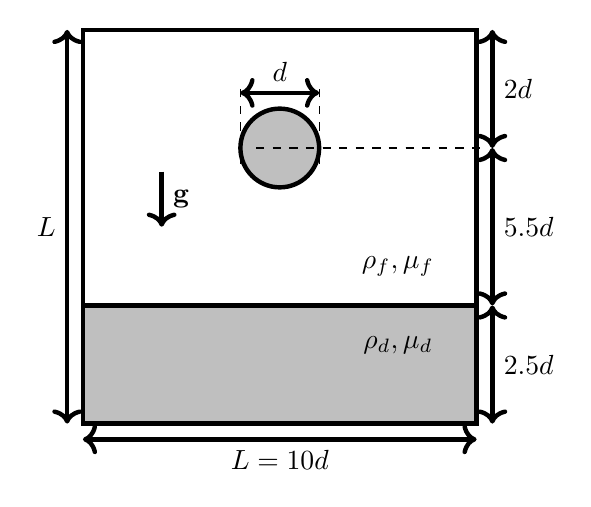
\begin{tikzpicture}[ultra thick]
        \draw (0,0) rectangle (5,5);
        \draw[fill=gray!50] (0,0) rectangle (5,1.5);
        \draw[fill=gray!50] (2.5,3.5) circle (0.5);
        \draw[<->](0,-0.2) --++ (5,0)node[midway,below]{$L  = 10 d$};
        \draw[<->](-0.2,0) --++ (0,5)node[midway,left]{$L$};
        \draw[<->](5.2,0) --++ (0,1.5)node[midway,right]{$2.5 d$};
        \draw[<->](5.2,1.5) --++ (0,2)node[midway,right]{$5.5 d$};
        \draw[<->](5.2,3.5) --++ (0,1.5)node[midway,right]{$ 2d$};
        \draw[dashed,thin](2.2,3.5) --++ (2.9,0);
        \draw[dashed,thin](2.2,3.5) --++ (2.9,0);
        \draw[->](1,3.2) --++ (0,-0.7)node[midway,right]{$\textbf{g}$};
        \draw[<->](2,4.2) --++ (1,0)node[midway,above]{$d$};
        \draw[thin,dashed](2,3.3) --++ (0,1);
        \draw[thin,dashed](3,3.3) --++ (0,1);
        \node (a) at (4,2){$\rho_f, \mu_f$};
        \node (a) at (4,1){$\rho_d, \mu_d$};
    \end{tikzpicture}
    \includegraphics[height = 0.4\textwidth]{image/VALIDATION2.0/Longmire/IMG/image-079.png}
    \caption{(left) Sketch of the computational set up at the initial time. 
    (right) Snapshot of the computational domain after the collision, with the pool interface represented in gray.
    The background color represents the velocity field magnitude, which is undisturbed, indicating a large enough domain. }
    \label{fig:schemeLong}
\end{figure}
\begin{figure}[h!]
    \centering
    \includegraphics[height = 0.3\textwidth]{image/VALIDATION2.0/Longmire/Re.pdf}
    \includegraphics[height = 0.3\textwidth]{image/VALIDATION2.0/Longmire/Dist.pdf}
    \caption{(left) Time evolution of the Reynolds number based on the droplet velocity, $Re(t) = \rho_fU d /\mu_f$ as a function of the dimensionless time, (+) numerical results of  \citet{balcazar2015multiple} (right)  position of the interfaces, ($\bullet$) top droplet surface, ($+$) bottom droplet surface, (x) pool surface. (Symbols) Experimental results of \citet{mohamed2003drop} (solid line) present numerical simulations with $d/\Delta = 20$. }
    \label{fig:resultslong}
\end{figure}
\ref{fig:resultslong} represents the comparison between our results and the experiment of \citet{mohamed2003drop} (right) and the numerical simulation of \citet{balcazar2015multiple} (left). 
The time-dependent Reynolds number as well as the interfaces positions are shown to closely match both the numerical and experiential results. 
From the very good agreement we conclude that the kinematics are well-represented even during contact for a mesh resolution of $d/\Delta = 20$.

\subsection{Mesh independence and statistical convergence for random arrays of drops}

Even though the aforementioned studies carried validations of the \texttt{Basilisk} code for rising droplets or bubbles, almost all of them considered isolated droplets or bubbles as the only validation case. 
To the author's knowledge, to this date no published study has presented a mesh independence study for random arrays of droplets or bubbles of this scale. 
As particle interactions and higher \textit{Galileo} numbers may be more challenging to model, it is primordial to investigate the mesh independence of the DNS that are carried in this work. 
In this objective we performed a DNS of a random array of $N_b=125$ droplets, with the following parameters
\begin{align*}
    \lambda = 10,
    && \zeta = 1.11,
    && Bo = 0.2,
    && Ga = 100,
    && \phi = 0.1,
    && N_b =125,
\end{align*}
with mesh resolutions of $d/\Delta = 5,\; 10,\; 18,\; 37$. 
This set of parameters have been selected following these arguments :
A viscosity ratio $\lambda = 10$ induces more vorticity at the droplets interfaces in contrast with the $\lambda = 1$ cases. 
For high inertia regimes ($Ga = 100$) the boundary layers at the droplet interfaces require the fine grid to be resolved compared to the low inertia cases. 
At $\phi = 0.1$, numerous interactions of droplets are present, implying that the good modeling of the liquid films between interfaces becomes predominant on the overall hydrodynamic, this also requires a good mesh resolution. 
% Additionally, the lower \textit{Bond} number employed here ($Bo=0.2$ instead of $Bo =0.5$) requires a higher mesh quality as well. 
For these reasons, we suppose that this case might require the finest grid among all other cases presented in this study. 
Based on this remark we can assume that if this case is mesh independent, then all cases from \ref{tab:simulations} are equally validated. 

Let us first verify the independence of the drift velocity on the mesh resolution. 
\begin{figure}[h!]
    \centering
    \includegraphics[height = 0.3\textwidth]{image/HOMOGENEOUS_NEW/VAL/tr.pdf}
    \includegraphics[height = 0.3\textwidth]{image/HOMOGENEOUS_NEW/VAL/Re.pdf}
    \caption{
        (left) Running average of the trace of $\textbf{R}$ as a function of the dimensionless time $t \sqrt{d/g}$. 
        (right) Running average of the Reynolds number based on the instantaneous volume-averaged relative velocity, $Re(t) = \rho_f U d /\mu_f$, with $U(t) = |\textbf{u}_d - \textbf{u}_c|$ for $\phi = 0.1$, $Ga=100$ and $\lambda =10$. 
        $\textbf{u}_d$ and $\textbf{u}_c$ represent the volume-averaged velocities of the dispersed phase and the continuous phase, respectively, at the dimensionless time $t \sqrt{d/g}$.
        %$\textbf{u}_p$ and $\textbf{u}_f$ are the particle and fluid phase volume averaged velocity at time $t$.
        In the legend we display the value of the mesh resolution. 
    }
    \label{fig:Re}
\end{figure}
In \ref{fig:Re} we display the running-averaged drift velocity as a function of time, for four mesh resolutions. 
The results are not as independent of the mesh resolution as the ordered array validation presented above. 
Indeed, we observe a difference of the rising Reynolds number of about $5\%$ between the $d/\Delta = 18$ and $d/\Delta = 37$ cases which is notable.
We recall that this $5\%$ error will eventually be lower for all other cases. 
The good agreement between the case  $d/\Delta = 10$ and $d/\Delta = 18$ is partially fortuitous.


% In \ref{fig:Re} (right) we display the running-averaged drift velocity as a function of time, for five mesh resolutions. 
% The results are not as independent of the mesh resolution as the ordered array validation presented above. 
% Indeed, we observe a difference of the rising Reynolds number of about $ 3\%$ between the $d/\Delta = 25$ and $d/\Delta = 60$ cases which is notable.
% We recall that this $3\%$ error will eventually be lower for all other cases. 

Now, let us turn our attention to \ref{fig:Re} (left), where we display the running average of $\text tr(\textbf{R})/r_m^2$ for different mesh resolutions.  
This figure validates two important points. 
First, we notice that the average of $\text tr(\textbf{R})/r_m^2$ appears well-converged at large $t\sqrt{d/g}$. 
This indicates that we have gathered a sufficient number of statistics to obtain accurate results. 
Secondly, it is found that the four cases converge approximately to the same value at large  $t\sqrt{d/g}$, implying that this quantity is also mesh-independent. 

\subsection{ Domain size independence study}

As discussed in the main text, the length scale of the distance between the particle layers is of the same order as the domain size. 
This raises an important question: Is the observed microstructure a physical phenomenon, or merely an artifact of the domain's size?
To address this, we conducted a DNS of a random array of $N_b=800$ droplets with a domain size of $\mathcal{L}/d = 20$. With the following dimensionless parameters:
\begin{align*}
    \lambda = 1,
    && \zeta = 1.11,
    && Bo = 0.5,
    && Ga = 80,
    && \phi = 0.05. 
\end{align*}
Note that the \textit{Galileo} number and the \textit{Bond} number are slightly different than in the original set of DNS due to numerical constraints.
We expect that these changes are not significant, so that the comparison remains valuable.


In \ref{fig:Pnst_large_domain} we compare the distribution $P_\text{nst}$ from the current case with $N_b =800$ droplets to the dataset used in this study with $N_b = 125$ droplets.
A good agreement is observed between the two distributions, although slight differences are noticeable.
These differences could be due to the different \textit{Galileo} numbers used in the larger simulation.
Nevertheless, the anisotropic behavior of $P_\text{nst}$ appears to be preserved between these two DNS.   
\begin{figure}[h!]
    \centering
    \includegraphics[height=0.205\textwidth]{image/HOMOGENEOUS_NEW/Dist/Pnst_l_1_Ga_100_PHI_0_05.pdf}
    \includegraphics[height=0.205\textwidth]{image/HOMOGENEOUS_final/Dist/Pnst_l_1_Ga_80_PHI_0_05.pdf}
    \caption{Histogram of the normalized function $P_\text{nst}$ at high inertia $Ga = 100$.
    The color map represents the values of the nearest pair distribution function. %of $P_\text{nst}$.
    The origin corresponds to the position of the \textit{\textit{test particle}}.
    The dimensionless radial and azimuthal coordinates, $|\textbf{r}|/d$ and $\theta$, correspond to the nearest neighbor position.
    The vertical direction corresponds to the flow direction, which is also the axis of symmetry for $P_\text{nst}$.
    (left) Original DNS with $N_b =125$ droplets.
    (right) Reference DNS with $N_b = 800$ droplets.}
    \label{fig:Pnst_large_domain}
\end{figure}
To provide a qualitative visualization of the system behavior, we displayed in \ref{fig:images_deux} a snapshot from both DNS. 
\begin{figure}[h!]
    \centering
    \includegraphics[width=0.45\textwidth]{image/HOMOGENEOUS_NEW/P_PHI_5_l_10_Ga_100.png}
    \includegraphics[width=0.45\textwidth]{image/HOMOGENEOUS_final/Ga_80_phi_005_l_1.png}
 %    \includegraphics[width=0.45\textwidth]{image/HOMOGENEOUS_NEW/Ga_100_phi_005_l_10.png}
    \caption{Snapshot of a simulation at $t^* = 150$ for $\phi=0.05$.
    Color map : values of the vertical component of the velocity, field on the vertical plane defined by the equation $z=0$. 
    (left)  Tipical DNS used in this study  with $\lambda = 1$ and $N_b = 125$ droplets.
    (right) A larger DNS with same $\phi$ and  $\lambda$ but with $N_b = 800$ droplets.
    }
    \label{fig:images_deux}
\end{figure}
We can observe that the DNS with $N_b = 800$ droplets also exhibits layers and clusters of droplets, similar to the original simulation. 
At this stage, we have not delved into quantitative analysis to verify if the distance between layers is consistent across both sets of simulations. 

Overall, we conclude that the domain size used in this work, $\mathcal{L}/d = 10$, is sufficient. 
Indeed, The distribution $P_\text{nst}$ remains similar in the larger domain (with $\mathcal{L}/d = 20$), and the microstructure displays the same types of particle layers and clusters.
%\subsection{Statistical convergence and mesh independence studies}
%
% \subsection{Statistical and mesh independence study}
\tb{Should i put the number of realization is abs $\omega$}

In the aim of providing accurate closure terms it is of primary importance to verify the well convergence of the mean quantities, either by varing the mesh definition domain size and duration of simulation.
To tackle this problem we carried out four simulation with 125 rising droplets with different mesh definition. 
The flow parameters for this validation read as,  
\begin{align*}
    \mu_r = 0.1,
    && \rho_r = 1.11,
    && Bo = 1,
    && Ga = 75,
    && \phi = 0.1,
    && N_b =125. 
\end{align*}
Note that in these simulations we used a number of $125$ droplets.  
In \ref{ap:A} we give more details on this choice and show that for our concerns it is a sufficient number of droplets. 

\ref{fig:Re_and_Tc}(left) display the cumulative mean of the vertical Reynolds number based on the drift velocity, namely,
\begin{equation}
    \widetilde{Re}(t)
    = \frac{\rho_f d}{\mu_f t}\int_{t_0}^{t_0+t} \left(\Xavg{\textbf{u}^0_d} -  \Xavg{\textbf{u}_c^0}\right)dt'
\end{equation}
\tb{ time average and volume average}
where $t_0$ is the starting sampling time. 
We remark a significant dependence of $\tilde{Re}$ with the mesh definition in contrast to the latter study (see \ref{fig:ordered_array}). 
It is hard to distinguish the cause of this difference, if it is not just because of the presence of interaction between droplets. 
Anyhow, we reach mesh independent results for $d/\Delta \geq 30$ in agreements with the recent studies of \citet{loisy2017buoyancy} \citet{zhang2021direct} for low inertial bubbly flows.
Also, $\widetilde{Re}$ reaches a constant values from $t^* = 50$. 
This is true for all mesh definition.  
Consequently, we reached an accurate time convergence for the rising velocity. 
\begin{figure}[h!]
    \centering
    % \includegraphics[height = 0.3\textwidth]{image/VALIDATION2.0/fCA/Re.pdf}
    \includegraphics[height = 0.3\textwidth]{image/VALIDATION2.0/fCA/Recum.pdf}
    \includegraphics[height = 0.3\textwidth]{image/VALIDATION2.0/fCA/Tcum.pdf}
    % \includegraphics[height = 0.35\textwidth]{image/VALIDATION2.0/fPA/Tcum.pdf}
    \caption{(left) Cumulative mean of the volume averaged Reynolds number along the simulation time based on the drift velocity $U = \textbf{u}_p - \textbf{u}_c$, with $\phi = 0.1$, $\rho_r = 1.11$, $ \mu_r =0.1$ and $Ga = 29.9$ and $N_b = 125$.
    (right) Cumulative mean of the fluid Reynolds stress tesor. }
    \label{fig:Re_and_Tc}
\end{figure}

The well convergence of the rising velocity doesn't guarantee a statistical nor a mesh convergence for finer quantities such as the pseudo-turbulent kinetic energy. 
Therefore, we provide on \ref{fig:UpUp} (left) the running average of the fluid phase pseudo-turbulent energy. 
Similarly, \ref{fig:UpUp} (right) represent the particle center of mass pseudo-turbulent kinetic energy. 
\begin{figure}[h!]
    \centering
    \includegraphics[height = 0.3\textwidth]{image/VALIDATION2.0/fCA/Tcum.pdf}
    \includegraphics[height = 0.3\textwidth]{image/VALIDATION2.0/fPA/Tcum.pdf}
    \caption{(left) Cumulative mean of the volume averaged granular temperature along the simulation time based on the drift velocity $U = \textbf{u}_p - \textbf{u}_c$, with $\phi = 0.1$, $\rho_r = 1.11$, $ \mu_r =0.1$ and $Ga = 29.9$ and $N_b = 125$.
    (right) Cumulative mean of the dimensionless particle-fluid-particle stress horizontal component tensor. }
    \label{fig:UpUp}
\end{figure}
Both figure exhibit well converged data. 
Interestingly, $\widetilde{K}_c$ and $\widetilde{K}_\alpha$ reach a constant value at $t^* = 200$ which is four time greater than for $\widetilde{Re}$.


\tb{this convergence can be compared to Loisy studies}
\tb{Cite and compare to Berner and \citet{bunner2002dynamics} which found that Nb > 12 is sufficient \citet{roghair2011drag}}
Now, let's investigate the required number of droplets per domain, $N_b$, and the minimum definition of cells per diameter of droplets $\delta$.  
\tb{Include bibliography and expectation here \ldots}
For this investigation we kept the physical parameters presented in the same section and made a double parametric analysis over $N$ and $\delta$. 
We carried out simulations for $N = 2, 3, 4, 5, 6, 7$, and for a number of cells $10 <\delta < 40$. 
In Basilisk the mesh definition is defined by a power of two, consequently depending on the size of the domain (which is fixed to keep a $\phi$ constant) the $\delta$ parameter is fixed at a power of 2 close. 
\begin{figure}[h!]
    \centering
    \includegraphics[height= 0.3\textwidth]{image/VALIDATION/N_and_delta/DUd.pdf}
    \includegraphics[height= 0.3\textwidth]{image/VALIDATION/N_and_delta/PHI.pdf}
    \caption{(left) Averaged Reynolds number based on the drift velocity.
            (right) Dispersed phase volume fraction at the end of each simulation.
            The text on the side of the points is $\delta$.
            N correspond to $N = N_b^3$. }
    \label{fig:VALIDATION_Nd_1}
\end{figure}
\ref{fig:VALIDATION_Nd_1}(left), illustrate clearly that the drift velocity is independent of the parameters $N_b$ and $\delta$, for $N >4$. 
On the other hand, \ref{fig:VALIDATION_Nd_1}(right), show that the volume fraction of the dispersed phase is lower for the low defined grid (red dots), due to a loss of volume during the simulation.
This doesn't mean that the solver isn't volume conservative. 
In fact, it is fund to be due to the \href{http://basilisk.fr/sandbox/fintzin/Rising-Suspension/no-coalescence.h}{no-coalescence.h} which generate fragment into the numerical domain, fragment which are deleted in the long run. 
\begin{figure}[h!]
    \centering
    \includegraphics[height= 0.3\textwidth]{image/VALIDATION/N_and_delta/PA_UpUp.pdf}
    \includegraphics[height= 0.3\textwidth]{image/VALIDATION/N_and_delta/Mh.pdf}
    \caption{(left) Fluids phase averaged fluctuation tensor.
            (right) Particular average of the first moment tensor, where $F_g$ is the buoyancy force applied on one droplet. 
            The numerical values displayed alongside the dots are the number of cells per diameter.}
    \label{fig:VALIDATION_Nd_2}
\end{figure}
Now, let's look at the behavior of more \textit{complicated} closure terms. 
\ref{fig:VALIDATION_Nd_2}(left) demonstrate that the vertical component of the pseudo turbulent tensor is parameter independent rather early, independently of the grid definition. 
This fact is rather surprising but note that the standard deviation is quite high for small domain. 
On \ref{fig:VALIDATION_Nd_2}(right), we can examine the vertical component of the first moment closure term. 
It is found to be constant for all $N$, but rather inaccurate for coarse grids. 
Which makes sens since the first moment results from a local calculation of the stress over a droplet volume, unlike the other quantities which results from the averaged center of mass velocity of a droplet. 

As we have shown, the quantities presented converge for a number of droplets equivalent to $N = 4$ and $\delta = 25$. 
Thus, we validate our simulation in space, i.e. we made sure that our domain were wide enough to minimize the influence of the periodicity on our results, and in mesh definition. 
Nevertheless, at it is the number of realization that matter when carrying a particular average, it is interesting to look at the duration of the simulation.


The last validation that we must expose is the convergence with the relative properties. 
Indeed, the film definition might change interaction properties such that the particle normal approach $\textbf{w}_n(a)$. 
\begin{figure}[h!]
    \centering
    \includegraphics[height=0.3\textwidth]{image/VALIDATION2.0/Hnst/ur_a_ndc_35_Ga_75.pdf}
    \caption{Normal approach Nearest particle velocity for different $Ga$. 
    We can see that for $\delta = 29,60$ we obtain the same results.}
\end{figure}




\bibliography{Bib/bib_bulles.bib}



\end{document}

